\section{Theorie}
\subsection{Grundlagen} \label{chap:Grundlagen}
Brechung findet statt, wenn eine elektromagnetische Welle mit einem elektrischen Feldvektor der Form 
\begin{equation}
    \vec{E}(\vec{r}) = \vec{E}_0 e^{i \vec{k} \vec{r} } 
\end{equation}
\begin{center}
    \tiny{( $ \vec{k} \hat{=} \text{Wellenvektor} $, $ \vec{r} \hat{=} \text{Ortsvektor} $ )}
\end{center}
von einem Medium mit Brechungsindex $n_1$ in ein Medium mit Brechungsindex $n_2$ ($n_1 \neq n_2$) übergeht. 
Bei der in diesem Versuch verwendeten Röntgenstrahlung handelt es sich dabei um eine elektromagnetische Welle mit einer Wellenlänge zwischen $\lambda = \SI{0,1}{\angstrom}$ und $\lambda = \SI{10}{\angstrom}$. \\
Der Brechungsindex kann als 
\begin{equation}
    n = 1 - \delta + i\beta
\end{equation}
\begin{center}
    \tiny{( $ \delta \hat{=} \text{Korrekturterm}\mathcal(O)10^{-6})) $, $ \beta \hat{=} \text{Absorbtion}\mathcal(O)(10^{-7} (\text{ für } E = \SI{6}{\kilo \electronvolt}   $ )}
\end{center}
geschrieben werden und ist für Röntgenstrahlung kleiner als eins.
Aus dem Snelliusschen Brechungsgesetz 
\begin{equation}
    \frac{n_1}{n_2} = \frac{\cos{\alpha_2}}{\cos{\alpha_1}}
\end{equation}
und der Annahme, dass es sich bei der Grenzfläche der Medien um eine homogene Ebene handelt, ergibt sich ein kritischer Winkel $\alpha_C$, bei dem es zur Totalreflektion kommt. Unter Vernachlässigung der Absorbtion folgt für kleine Winkel näherungsweise
\begin{equation}
    \alpha_c \approx \sqrt{2 \delta} = \lambda \sqrt{ \frac{r_e \rho}{\pi} } .
\end{equation}
\begin{center}
    \tiny{( $ r_e \hat{=} \text{Klassischer Elektronenradius} $, $ \rho \hat{=} \text{Elektronendichte des Materials}$ )}
\end{center}

\subsection{Fresnel Formeln}
Im allgemeinen muss bei der Reflektion und Transmission elektromagnetischer Wellen die Polarisation des Lichts berücksichtigt werden. Dies geschieht mithilfe der Fresnel Formeln. Für s-polarisiertes Licht ergeben sich
\begin{align}
    r &= \frac{n_1 \cos{\alpha_1} - n_2 \cos{\alpha_2} }{n_1 \cos{\alpha_1} + n_2 \cos{\alpha_2} }\\
    t &= \frac{2 n_1 }{n_1 \cos{\alpha_1} + n_2 \cos{\alpha_2} }.
\end{align}
Für diesen Versuch ist eine Unterscheidung zwischen $p$ und $s$ Polarisation aufgrund der ähnlichen Brechungsindizes $n_1 \approx n_2$ nicht nötig. 
Die Fresnel Fresnelreflektivität ist für Röntgenstrahlung und für $ \alpha_i > 3\alpha_c$ näherungsweise
\begin{equation}
  R_f = \left( \frac{\alpha_c}{2 \alpha_i} \right)  . 
\end{equation}

\subsection{Mehrschichtsysteme}
Da in diesem Versuch mit Polystyrolschicht auf einem Siliziumsubstrat gearbeitet wird, wird im folgendem
der Umgang mit Mehrschichtsystemen erläutert. Ein beispielhaftes Verhalten der Refletivität befindet sich in Abbildung \ref{fig:reflectivity}. 

\begin{figure}[H]
    \centering
    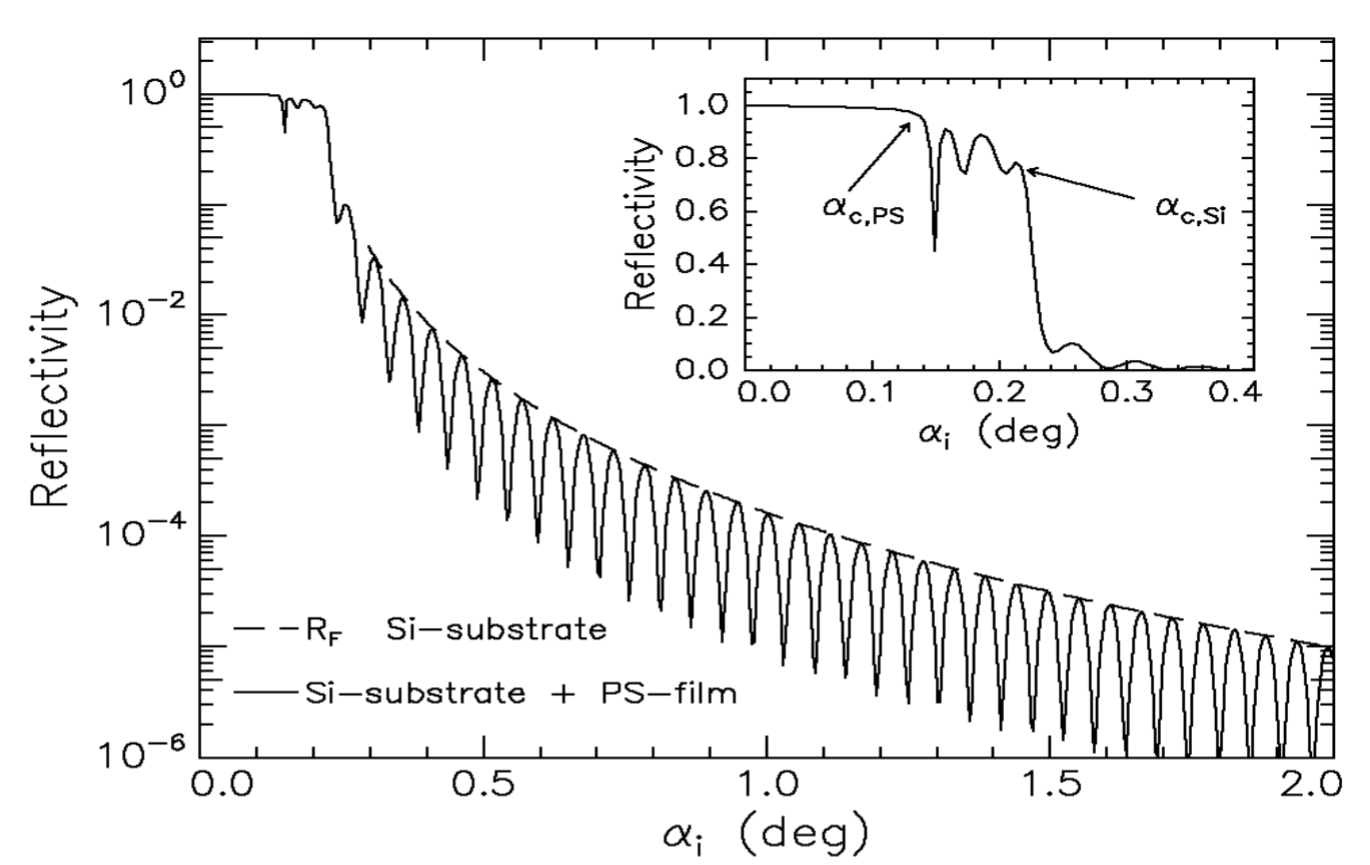
\includegraphics[width = 0.8 \textwidth]{content/images/reflectivity.png}
    \caption{Beispielhafte Auftragung der Röntgenreflektivität R gegen den Einfallswinkel $\alpha_i$ \cite{e1}. }
    \label{fig:reflectivity}
\end{figure}

In dem dort vergrößerten Bereich sind zwei Totalreflektionen zu erkennen. Bei diesen handelt es sich um die Totalreflektionen von Silizium und des Polystyrolfilm. Für höhere Einfallswinkel folgt der zu erwartene Abfall der Refletivität. Die dabei beobachtbaren Oszillationen treten aufgrund von Interferenteffekten an der Oberfläche auf. Mithilfe dieser Oszillationen lassen sich Rückschlüsse auf den Schichtabstand ziehen, da der Gangunterschied für destruktive Interferenzen ein ungerades Vielfaches von $\frac{\lambda}{2}$ sein muss. 
Damit folgt der Zusammenhang
\begin{equation}
    d = \frac{2 \pi}{\delta q_z} = \frac{\lambda}{2\delta \alpha_1} .
\end{equation}
\begin{center}
   \tiny{ ($\vec{q} = \vec{k_2}-\vec{k_1}$, $ q_z = 2k \sin{\alpha_1} $ ) }    
\end{center}
Handelt es sich nun bei dem zu betrachtenem System um - wie in Abbild \ref{fig:layer} dargestellt - ein System mit N+1 Schichten, kann die Reflektivität mithilfe des rekursiven Parratt-Algorithmus berechnet werden. Dieser trifft die Annahme, dass es sich bei der untersten Schicht um eine unendlich dicke Schicht handelt, sodass an dieser keine Transmission stattfindet. 

\begin{figure}[H]
    \centering
    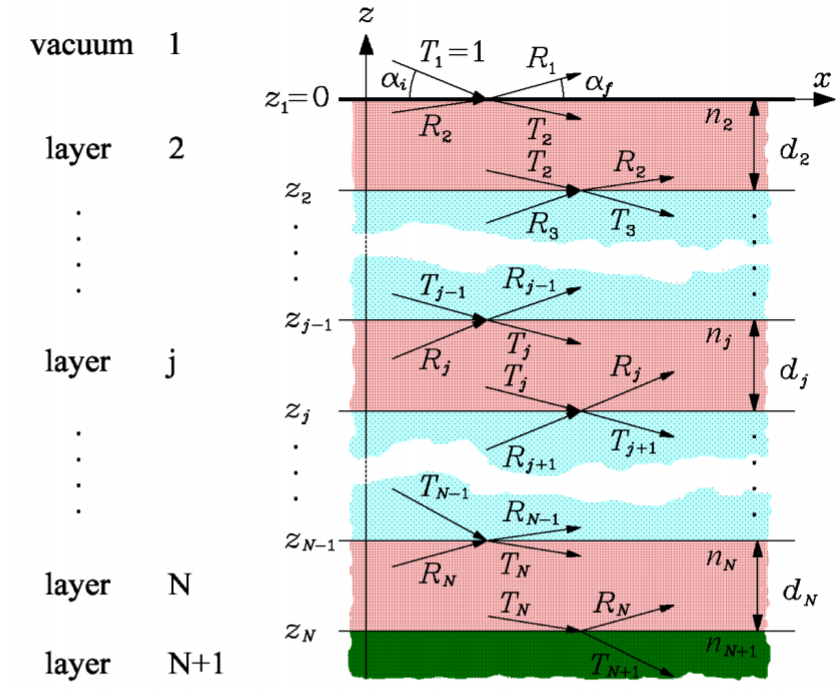
\includegraphics[width = 0.8 \textwidth]{content/images/layers.png}
    \caption{Beispielhafte Darstellung eines Mehrschichtensystems mit N+1 Schichten \cite{e1}. }
    \label{fig:layer}
\end{figure}


\subsection{Rauigkeit}
Im Kapitel \ref{chap:Grundlagen} wurde angenommen, dass es sich bei den Oberflächen perfekt glatte Oberflächen handelt. Da dies im Experiment jedoch nicht der Fall ist, muss dies bei der Berechnung der Reflektivität berücksichtigt werden. 
Dafür werden die modifizierten Fresnelkoeffizienten
\begin{align}
    \tilde{r}_{j,j+1}&=r_{j,j+1}\exp(-2k_{z,j}k_{z,j+1}\sigma^2_j)\\
    \tilde{t}_{j,j+1}&=t_{j,j+1}\exp((k_{z,j-k_{z,j+1}})^2 \cdot \frac{\sigma^2_j}{2})
\end{align} 
genutzt. %Der Einfluss der Rauigkeit ist in Abbildung \ref{fig:rau} dargestellt. 

\subsection{Geometriefaktor und Geometriewinkel}
Wie in Abbildung \ref{fig:geo} zu sehen ist, überstreicht der verwendete Strahl eine größere Fläche, als die Probenoberfläche. Dies führt dazu, dass nur ein Teil der Intensität $I$ reflektiert und somit später detektiert wird. 
Dies wird durch den Geometriefaktor G berücksichtigt und wird als das Verhältnis der Strahlbreite
$D \sin{\alpha_i} $, die die Probenoberfläche trifft, zur Gesamtstrahlbreite $d_0$ defniert.
Dabei gilt:
\begin{align}
    G&=\frac{D\sin\alpha_i}{d_0}\;\;\; &\text{mit}\;\;\; &\alpha_i<\alpha_g\;\;\; \text{und}\\
    G&=1\;\;\; &\text{mit}\;\;\; &\alpha_i>\alpha_g.
\end{align}

\begin{figure}
    \centering
    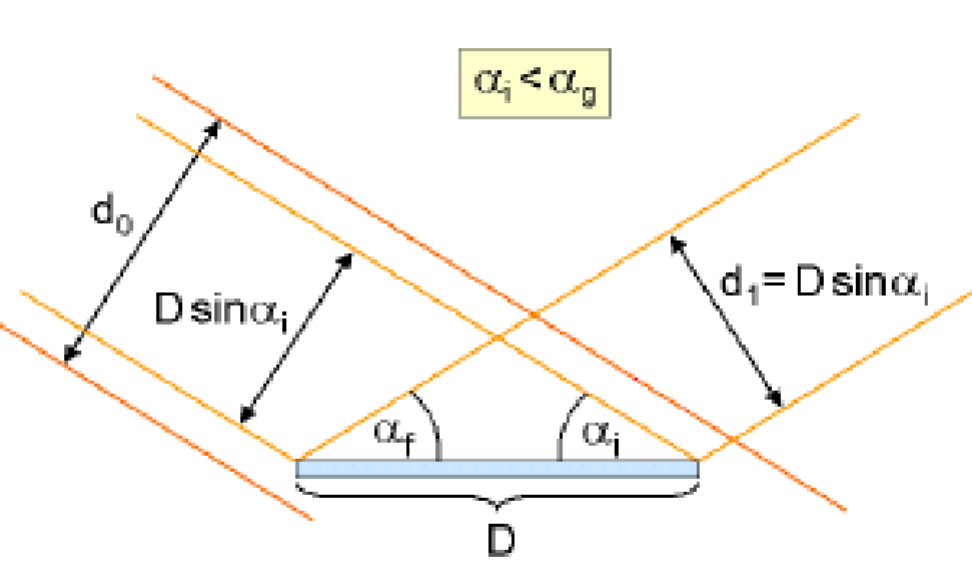
\includegraphics[width=0.6\textwidth]{content/images/Geometriewinkel.png}
    \caption{Veranschaulichung des Geometriewinkels \cite{anleitung}.}
    \label{fig:geo}
  \end{figure}